\chapter{Evaporadores}
\section{Generalidades}


	El evaporador es el componente del sistema de refrigeración utilizado para absorber el calor del ambiente y transferirlo al refrigerante que circula por su interior. Está compuesto por tubos, pasajes o recipientes hechos generalmente de cobre o aluminio para diámetros pequeños y de cobre y acero para diámetros grandes.
	
	
	
%	Absorbe el calor debido al refrigerante contenido en los tubos. Contiene, además, un fluido (o producto refrigerante) que está separado del refrigerante por las paredes o carcasa del intercambiador.
	
	\section{Clasificación}
	\subsection{Clasificación según su construcción}
	
		Existen tres tipos generales de evaporadores
		\begin{itemize}
			\item de tubos desnudos,
			\item de superficie extendida,
			\item y de placas.
		\end{itemize}
	
		\subsubsection{Evaporadores de tubos desnudos}
		
			Están formados por tubos (generalmente de cobre o acero) sin aletas ni elementos que aumenten la superficie de transferencia de calor.
			\begin{figure}[h]
				\centering
				\begin{subfigure}{.4\linewidth}
					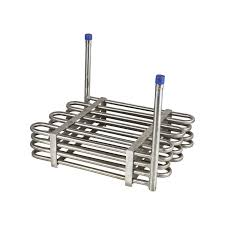
\includegraphics[width=\linewidth]{evaporadores/evaporador-tubo-1}
					
				\end{subfigure}
			\begin{subfigure}{.4\linewidth}
				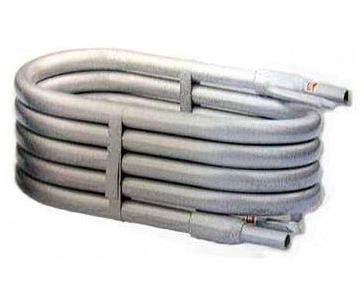
\includegraphics[width=\linewidth]{evaporadores/evaporador-tubo-2}
				
			\end{subfigure}
			\caption{Evaporadores de tubo.}
			\label{fig:evaporadores-tubo}
			\end{figure}
			
			Los tubos de acero se utilizan en evaporadores grandes y en evaporadores que utilicen amoníaco como refrigerante, mientras que los tubos de cobre se emplean en evaporadores pequeños y se los usa con refrigerante que no sea amoníaco.
			
			Estos evaporadores se forman en una amplia variedad de tamaños, forma y diseños, y es muy común que sean fabricados a la medida según el diseño.
	
		\subsubsection{Evaporadores de superficie extendida}
		
			Están formados por un serpentín de tubería en la que se aplican aletas de aluminio para aumentar la superficie de transmisión del propio tubo.
			
			\begin{figure}[h]
				\centering
				\begin{subfigure}{.4\linewidth}
					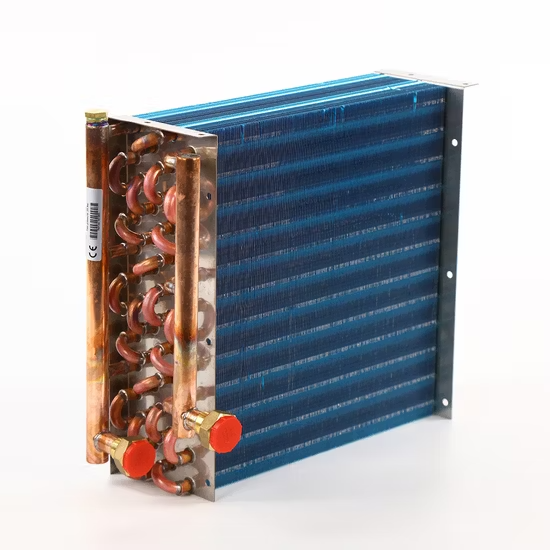
\includegraphics[width=\linewidth]{evaporadores/evaporador-superficie-1}
				\end{subfigure}
			\begin{subfigure}{.4\linewidth}
				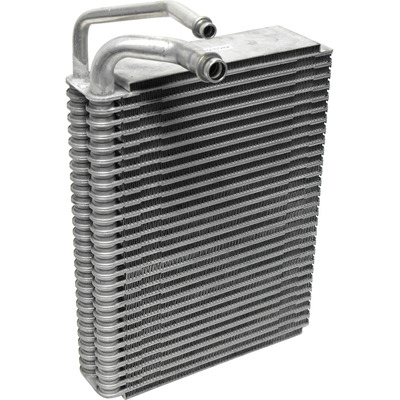
\includegraphics[width=\linewidth]{evaporadores/evaporador-superficie-2}
			\end{subfigure}
			\caption{Evaporadores de superficie extendida.}
			\label{fig:evaporadores-superficie}
			\end{figure}
			
			Cuando se agregan aletas al serpetín, éstas se extienden hacia afuera y actúan como colectores de calor. Aboserben calor del aire que ordinariamente no estaría en contacto con la superficie de los tubos desnudos, y conducen este calor hacia la tubería.
			
			
			Para que las aletas sean eficientes deberán estar unidas a la tubería de manera tal que se asegure un buen contacto térmico. En algunos casos las aletas están soldadas directamente a los tubos, mientras que en otros casos, las aletas se hacen deslizar sobre la tubería y se expande a esta última, por lo que permite una correcta sujeción.
		
		
			El tamaño del tubo determina el tamaño de la aleta, y el espaciamiento entre cada una de ellas varía según el tipo de aplicación. Para aplicaciones a muy bajas temperaturas, se produce un inevitable acumulamiento de escarcha entre las aletas, lo que tiende a restringir el paso de aire a través del serpentín. Es por ese motivo que para este tipo de aplicaciones, los evaporadores deberán tener un mayor espaciamiento (dos o tres aletas por pulgada) a fin de minimizar daños por la restricción en la circulación del aire. Mientras que, para aplicaciones donde los serpentines trabajan a temperaturas suficientemente altas, de tal modo que no se produzca escarcha sobre la superficie, podrán tenerse hasta 14 aletas por pulgada. No obstante, un aleteado excesivo podrá reducir la capacidad del evaporador porque restringiría innecesariamente la circulación de aire a través del serpentín.
		
			
			
		
		\subsubsection{Evaporadores de placas}
		
		
			Consisten en la unión de dos placas unidas herméticamente con un circuito trazado en su interior por donde circulará el refrigerante.
			
			La superficie plana de las placas pueden ser fabricadas en una diversidad de formas y los pasajes de refrigerantes pueden ser integrales o adheridos. Algunos son construidos con dos placas planas de metal realzadas y soldadas una con otra de tal modo que pueda fluir el refrigerante entre ambas, mientras que en otros se tiene una tubería instalada entre dos placas metálicas las cuales están soldadas por sus orillas.			
			
			\begin{figure}[h]
				\centering
				\begin{subfigure}{.4\linewidth}
				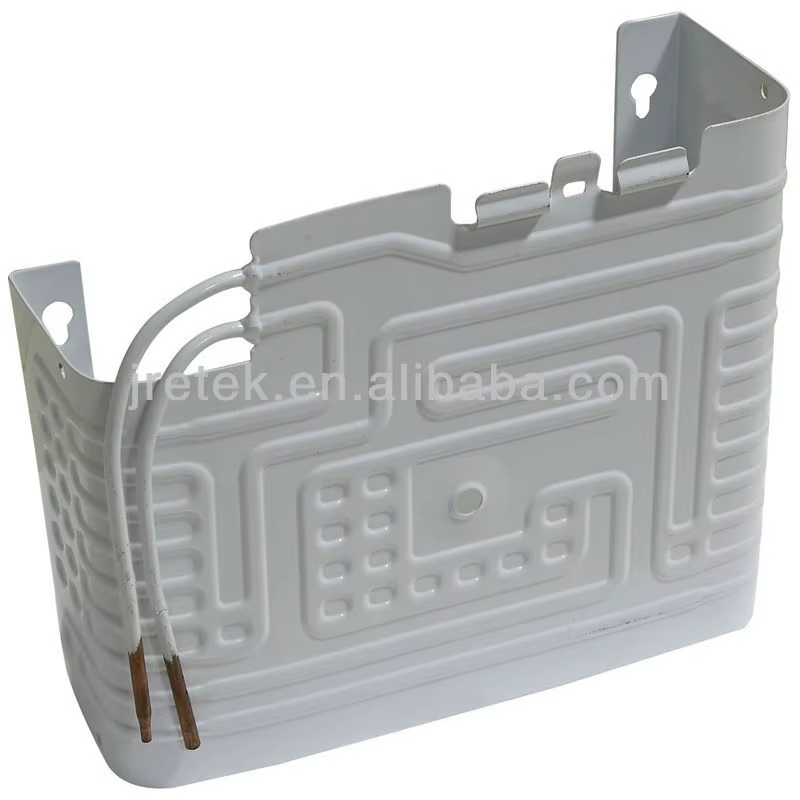
\includegraphics[width=\linewidth]{evaporadores/evaporador-placa-1}
				\end{subfigure}
				\begin{subfigure}{.4\linewidth}
				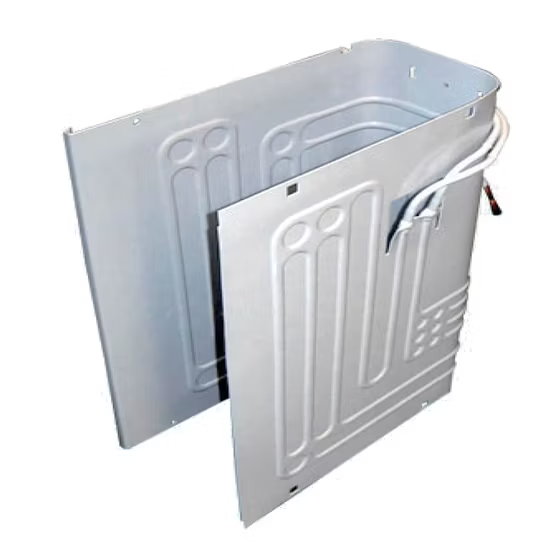
\includegraphics[width=\linewidth]{evaporadores/evaporador-placa-2}
				\end{subfigure}
				\caption{Evaporadores de placa.}
				\label{fig:evaporadores-placa}
			\end{figure}
	
	\subsection{Clasificación según la circulación del aire}	
	
	La circulación de aire en un espacio refrigerado es esencial para la transferencia de calor del producto hacia el evaporador. En productos que no están envasados a prueba de vapor, la inadecuada circulación puede ser determinante. Cuando la circulación de aire es muy grande, se aumenta la rapidez de evaporación de la humedad lo que produce una deshidratación en el producto. Mientras que, una escasa circulación de aire favorece el crecimiento de hongos y bacterias. Por otra parte, cuando el producto está envasado a prueba de vapor no se verá afectado por altas velocidades y la velocidad de circulación de aire se debe mantener en un nivel alto para obtener un efecto de enfriamiento máximo.
	
	La circulación de aire deseada varía con las diferentes aplicaciones y depende sobre todo de la humedad del espacio, del tipo de producto y del período de tiempo de almacenaje. 
	
	Los evaporadores se pueden clasificar según la circulación de aire sobre el serpentín en evaporadores de \emph{convección natural} y de \emph{convección forzada}.
	
	\subsubsection{Evaporadores de convección natural}
	
	Se usan frecuentemente en aplicaciones donde se desea aire de baja velocidad y deshidratación mínima del producto. Son instalaciones típicas las que se tienen en unidades de exhibición, enfriadores con pasillo interior y en cuartos grandes de almacenaje. En la \autoref{fig:conveccion-natural} se muestra un evaporador de este tipo.
	
	
	\begin{figure}[h]
		\centering
		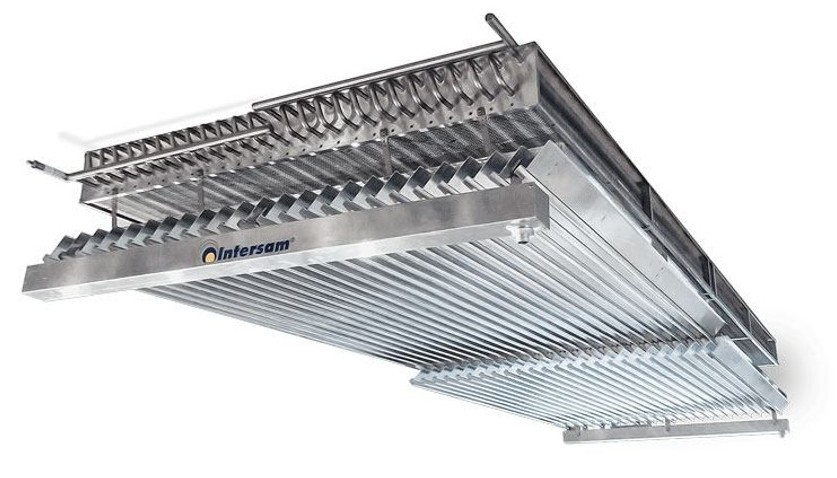
\includegraphics[width=.5\linewidth]{evaporadores/natural}
		\caption{Evaporador de techo de convección natural.}\label{fig:conveccion-natural}
	\end{figure}
	
	La circulación de aire sobre el serpentín se da por el diferencial de temperatura y densidad del aire entre el evaporador y el espacio. A mayor diferencia de temperatura, mayor será la velocidad de circulación del aire. Esta depende de la forma, tamaño y localización del evaporador, por el uso de desviadores y por la colocación del producto en el espacio.
	
	A causa de que el movimiento de aire es por el fenómeno de convección natural, el consumo en este tipo de instalaciones es menor respecto al de convección forzada.
	
	\subsubsection{Evaporadores de convección forzada}
	
	Conocidos comercialmente por el nombre de \emph{unidad enfriadora}, se caracterizan por estar equipados con ventiladores para forzar la circulación de aire sobre el serpentín. La \autoref{fig:conveccion-forzada} muestra un ejemplo de evaporador con dos ventiladores.
	
	\begin{figure}[h]
		\centering
		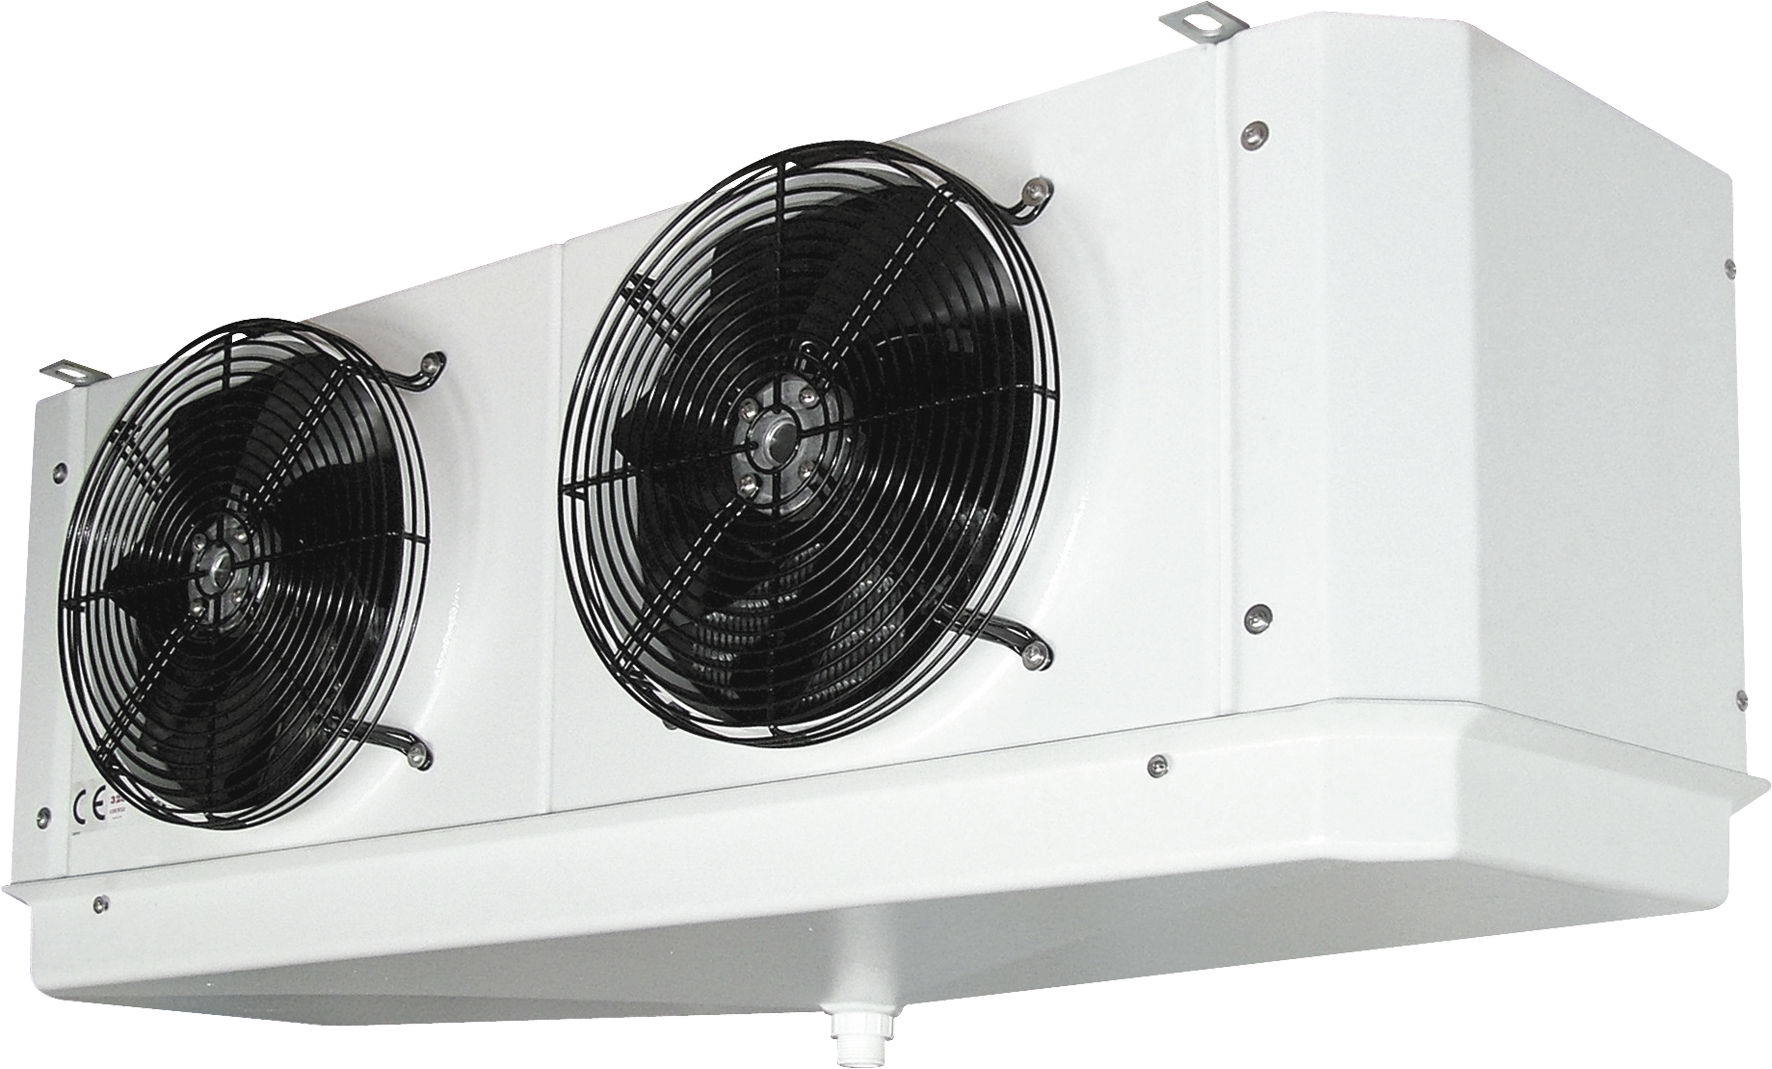
\includegraphics[width=.5\linewidth]{evaporadores/forzados}
		\caption{Evaporador de convección forzada.}\label{fig:conveccion-forzada}
	\end{figure}
	
	\subsection{Clasificación según el método de alimentación del refrigerante}
		
		Los evaporadores también pueden ser clasificados de acuerdo al método de alimentación del líquido refrigerante como evaporadores de \emph{expansión seca}, \emph{inundados} y \emph{sobrealimentados}.
		
		
			\subsubsection{Evaporador de expansión seca}
				
				Como se observa en la \autoref{fig:expansion-directa}, en el evaporador de expansión seca la mezcla de gas y líquido refrigerante que sale de la válvula de expansión entra directamente al serpentín. Parte de la masa, la que se encuentra en fase líquida, se vaporiza progresivamente a medida que el refrigerante pasa a través del evaporador.
			
			
				Los evaporadores de expansión seca son menos eficientes que los de otro tipo, pero son por lo general mucho más simples en su diseño, más económicos, requieren menos carga de refrigerante y tienen menos problemas que los demás en lo que respecta al regreso del aceite. Por estas razones, los evaporadores de expansión seca son el tipo más popular.
				
				
				\begin{figure}[h]
					\centering
					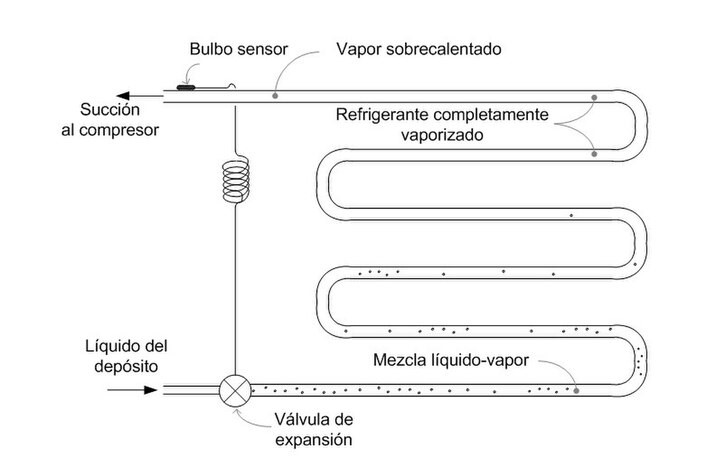
\includegraphics[width=.7\linewidth]{evaporadores/expansion-directa}
					\caption{Evaporador de expansión seca.}
					\label{fig:expansion-directa}
				\end{figure}
		
		
			\subsubsection{Evaporador inundado}
			
				Los evaporadores inundados se llenan completamente con el refrigerante líquido a fin de tener humedecida toda la superficie interna del tubo, y en consecuencia, la mayor razón posible de transferencia de calor.
				
				Como se muestra en la \autoref{fig:inundado}, el evaporador está equipado con un acumulador o colector de vapor que sirve como receptor de líquido, desde el cual solo el refrigerante líquido es circulado por gravedad a través del serpentín. 
				
				El vapor generado por la ebullición del refrigerante en los tubos del evaporador y el vapor flash, se separan del líquido en la parte superior del acumulador de donde es sacado directamente a través de la línea de succión para continuar su ciclo hacia el compresor.
				
				
				\begin{figure}[h]
					\centering
					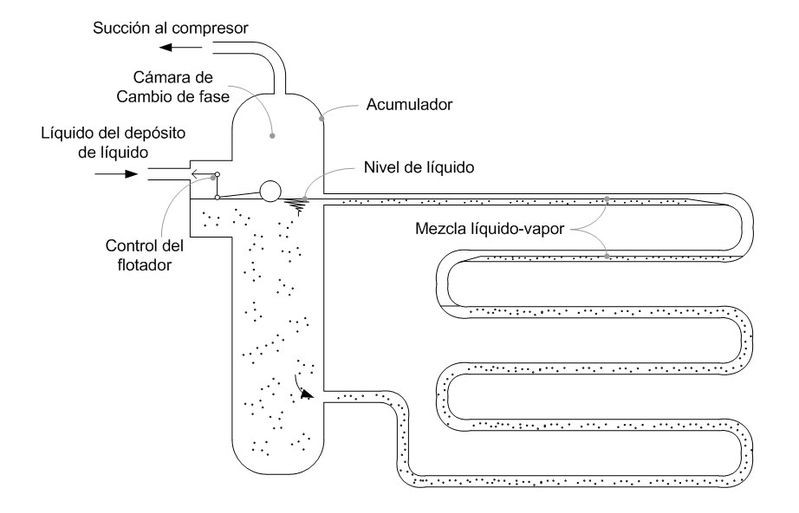
\includegraphics[width=.7\linewidth]{evaporadores/inundado}
					\caption{Evaporador inundado.}
					\label{fig:inundado}
				\end{figure}
		
			\subsubsection{Evaporador sobrealimentado}
			
				Los evaporadores sobrealimentados son un tipo especial del sistema de evaporador inundado, también se denominan como evaporadores recirculados o de circulación forzada. Cuentan con una bomba para forzar la circulación del refrigerante a través del serpentín. Son más comunmente empleados en sistemas de evaporador múltiple, como se ve en la \autoref{fig:sobrealimentado}.
		
				\begin{figure}[h]
					\centering
					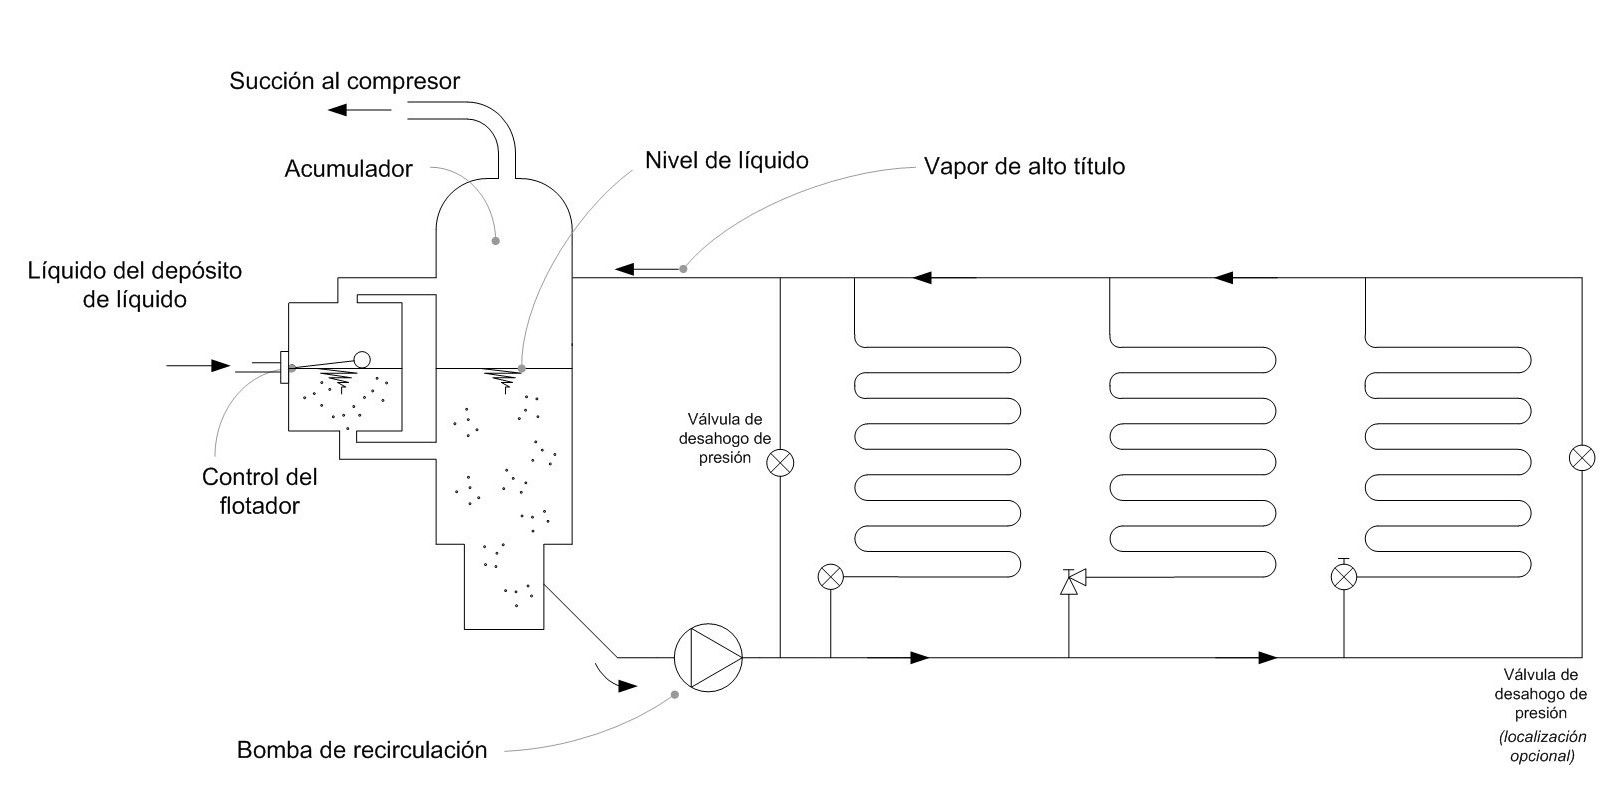
\includegraphics[width=.9\linewidth]{evaporadores/sobrealimentado}
					\caption{Evaporador de líquido sobrealimentado.}
					\label{fig:sobrealimentado}
				\end{figure}
				
				En este tipo de sistema se minimizan los problemas relacionados con el retorno de aceite en el evaporador. Además, a diferencia del sistema inundado en el que líquido refrigerante circula por acción de la gravedad, el sistema sobrealimentado presenta la ventaja de que el tanque acumulador no requiere estar ubicado necesariamente por encima del evaporador.
		
	\subsection{Clasificación según la transmisión del frío}
	
			Los sistemas se pueden clasificar según la forma en la que el espacio es refrigerado en sistemas \emph{directos} e \emph{indirectos}.
			
			\subsubsection{Sistemas directos}
				
			Un sistema de refrigeración por expansión directa, también llamado de refrigeración directa, es aquel en el que el refrigerante circula por el evaporador y entra en contacto directo con el medio o el espacio que se desea enfriar, sin utilizar un fluido intermedio. Este tipo de sistema es común en heladeras, aires acondicionados y cámaras frigoríficas pequeñas por su eficiencia y simplicidad.
				
			\subsubsection{Sistemas indirectos}
				
				Los sistemas de refrigeración indirecta emplean agua o salmuera empleadas como \emph{refrigerante secundario} para refrigerar el espacio. El refrigerante primario enfría al secundario y luego este se dirige para entrar en contacto directo con el espacio o producto a refrigerar.
				
				Estos sistemas se emplean cuando el lugar a refrigerar está a una distancia considerable del equipo de condensación. El uso del sistema indirecto evita problemas como el retorno de aceite y las excesivas caídas de presión en las tuberías. Además, las fugas causan problemas serios y es más fácil de que ocurran en tuberías con refrigerante que en tuberías con agua o salmuera. Por otra parte, son empleados con ventaja en instalaciones donde la fuga del refrigerante y/o aceite pueda contaminar al producto, como en plantas empacadoras de carne o en grandes aplicaciones de almacenes fríos en los cuales se usa amoníaco como refrigerante primario.
				
				Algunos refrigerantes secundarios son agua, cloruro de calcio y salmueras como cloruro de sodio, flicoles de etileno y propileno, y metanol.
		
	\section{Capacidad del evaporador}\label{sec:capacidad-evaporador}
	
		El calor puede llegar al evaporador por los tres métodos de transferencia de calor conocidos. De todas maneras, éste debe pasar por \emph{conducción} al refrigerante en el interior a través de las paredes del evaporador. La cantidad de calor transferido por conducción a través de cualquier superficie se expresa como
		
		\begin{equation}\label{eq:calor}
			Q = A \cdot U \cdot D
		\end{equation}
		
		Donde \begin{itemize}
			\item $Q$ es la cantidad de calor transferido por hora,
			\item $A$ es el área de la superficie exterior del evaporador,
			\item $U$ es el coeficidente total de transferencia,
			\item $D$ es la diferencia de temperatura media logarítmica entre la temperatura del evaporador y la temperatura del refrigerante.
		\end{itemize}
	
	
			\subsection{Coeficiente total de transferencia}
				
				La resistencia al flujo de calor ofrecida por las paredes del evaporador es suma de tres factores, cuya relación queda expresada como
				
				\begin{equation}\label{eq:conductancia-total}
					\dfrac{1}{U} = \dfrac{R}{f_i} + \dfrac{L}{k} + \dfrac{1}{f_o}
				\end{equation}
				
				donde \begin{itemize}
					\item $U$ es el coeficiente total de transferencia,
					\item $L/k$ es la resistencia al flujo de calor ofrecida por el metal de los tubos y aletas,
					\item $R$ es la relación de superficie exterior a superficie interior,
					\item $f_i$ es el factor de conductancia de la película de la superficie interior,
					\item $f_o$ es el factor de conductancia de la película de la superficie exterior.
				\end{itemize}
				
				El coeficiente total de transferencia deberá ser lo más grande posible para tener una alta transferencia de calor a través de las paredes del evaporador. Generalmente, se emplean metales para la construcción de los evaporadores. Sin embargo, debe tenerse en consideración el tipo de refrigerante que se emplee para evitar reacciones no deseadas con el metal. 
		
				
				Los metales que se usan con mayor frecuencia, son: hierro vaciado, acero, cobre, latón y aluminio. El hierro vaciado y el acero no se ven afectados por ninguno de los refrigerantes más comunes, no obstante, se oxidan al haber humedad en el sistema. El latón y el cobre pueden usarse con cualquier refrigerante menos con el amoníaco, el cual disuelve el cobre. El aluminio puede utilizarse con cualquier refrigerante menos con el cloruro de metilo.\\
				
				De los tres términos involucrados en la \autoref{eq:conductancia-total}, aquellos que involucran los coeficientes de conductancia de las superficies de película son los mayores y, por tanto, de mayor interés.
				
				
				En relación con esto, la transferencia de calor por conducción es mayor a través de líquidos que a través de gases, y la rapidez a la cual el refrigerante transfiere calor incrementa a medida que lo hace la superficie humedecida. En este aspecto, los evaporadores inundados, dado que están completamente llenos de líquido, son más eficientes que los del tipo expansión seca. Este principio también se aplica a la superficie externa del evaporador.
		
		
				Cualquier suciedad que se tenga ya sea en las superficies externas o internas, tienden a actuar como aislamiento térmico y a diminuir el factor de conductancia. El aislamiento externo o suciedad en la superficie externa del evaporador puede deberse a
				
				\begin{itemize}
					\item la suciedad originada por polvos que lleva el aire y se adhieren a la superficie,
					\item la formación de incrustaciones y a la oxidación,
					\item la formación y acumulación de escarcha.
				\end{itemize}
				
				La suciedad en la superficie interna de los tubos del evaporador se puede originar por
				
				\begin{itemize}
					\item cantidades excesivas de aceite en el evaporador,
					\item bajas velocidades del refrigerante, generando acumulación de burbujas debido a la acción de ebullición del fluido.
				\end{itemize}
				
				En relación con la velocidad del fluido, la conductancia de la película en la superficie puede mejorarse al aumentar la velocidad del fluido. Sin embargo, en el interior de los tubos, la velocidad está limitada por la máxima caída de presión admisible a través del serpentín. Mientras que, la velocidad del fluido sobre la superficie externa del serpentín está limitada por otras consecuencias que no son en sí mismo la capacidad del evaporador.
				
				
				\emph{Cualquier incremento que se tenga en la turbulencia del flujo, ya sea dentro o fuera del evaporador, aumentará considerablemente la tasa de transferencia de calor a través de las paredes del evaporador}. 
				
				En general, la tuberbulencia interna se aumenta con la diferencia de temperatura a través de las paredes del tubo. La turbulencia externa está influida por la velocidad del fluido sobre el serpentín, por el espaciamiento de los tubos y por la forma de las aletas.\\
				
			\subsection{Ventajas de usar aletas}
				
				La ventaja del aleteado depende de los coeficientes de conductancia de las superficies de película exterior e interior, y de la relación $R$ entre dichos valores. 
				
				
				% Acá habla de la tasa de transferencia de calor en las superficies. Tengo entendido que esto funciona como un cuello de botella: se espera que ambas superficies, externa e interna, tengan la misma tasa. Sin embargo, en instalaciones de aire, la superficie interna tiene una tasa mayor por lo que se aumenta la superficie externa con aleteados para incrementar la externa. Mientras que, en instalaciones donde el serpentín está en contacto con líquido se utilizan tubos desnudos.
				En instalaciones de refrigeración de aire la rapidez de flujo de calor en la superficie exterior es menor que la de superficie interior, por lo que la capacidad total del evaporador estará limitada por la capacidad de la superficie exterior. Para estos casos, el valor total de $U$ puede incrementarse usando aletas para aumentar el área de la superficie exterior hasta un valor tal que la cantidad de calor absorbido por la superficie exterior sea aproximadamente igual a la que pueda pasar por la superficie interior. Por otra parte, en aplicaciones donde el líquido esté en contacto en ambos lados del tubo y en los que la transferencia de calor es aproximadamente igual para ambas superficies, los evaporadores de tubo descubierto muestran una alta eficiencia y el aleteado no es necesario.	\\
		
				En algunas instalaciones con enfriamiento de líquido que utilizan refrigerantes fluorocarburos, la rapidez de transferencia de calor sobre el lado del fluido enfriado puede exceder a la rapidez sobre el lado del refrigerante, en cuyo caso el aleteado del tubo en el lado del refrigerante mejorará el rendimiento del evaporador. En la \autoref{fig:aleteado-interno} se muestran varios ejemplos de aleteado interno.
			
				\begin{figure}[h]
					\centering
					% Columna izquierda - subfigura (a)
					\begin{subfigure}{0.58\linewidth}
						\centering
						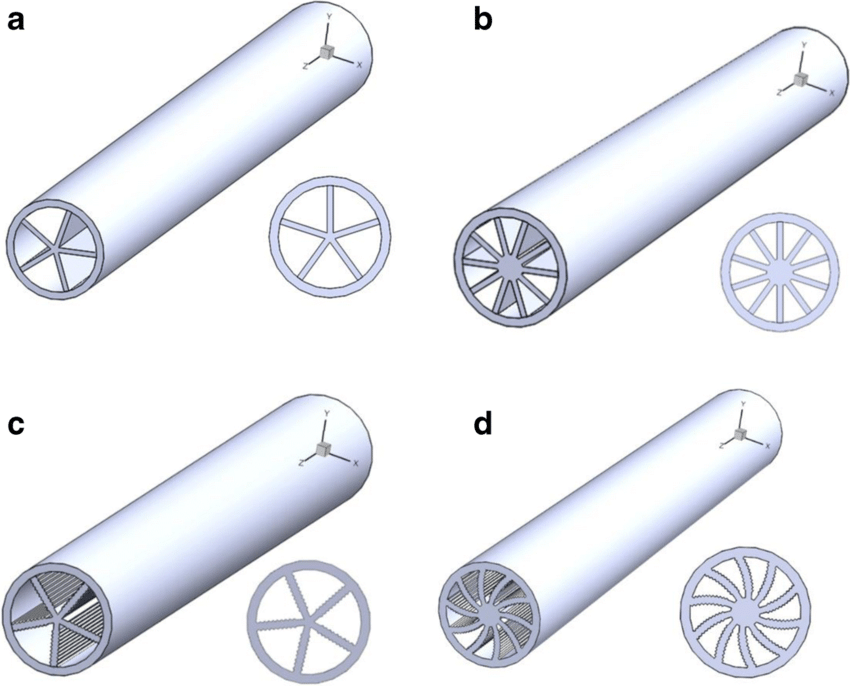
\includegraphics[width=\linewidth]{evaporadores/aleteado-interno-1}
					\end{subfigure}
					% Columna derecha con subfigura (b) y (c)
					\begin{subfigure}{0.3\linewidth}
						\centering
						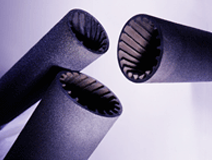
\includegraphics[width=\linewidth]{evaporadores/aleteado-interno-2}
						
						\vspace{0.3cm}
						
						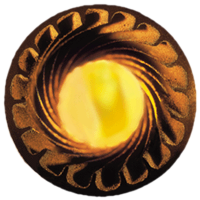
\includegraphics[width=.7\linewidth]{evaporadores/aleteado-interno-3}
					\end{subfigure}
					
					\caption{Algunos ejemplos de aleteado interno.}
					\label{fig:aleteado-interno}
				\end{figure}
			
			\subsection{Diferencia de temperatura media logarítmica}
			
				La diferencia de temperatura media real del aire, también conocida como temperatura efectiva media (METD), se obtiene como el promedio logarítmico entre las temperaturas de entrada y salida del aire. Se calcula según la \autoref{eq:metd}, asumiendo que la temperatura del refrigerante ($T_r$) se mantiene constante durante el proceso.
				
				\begin{equation}\label{eq:metd}
					D = \dfrac{(T-e - T_r) - (T_s - T_r)}{\ln\dfrac{T_e - T_r}{T_s - T_r}}
				\end{equation}
				Donde\begin{itemize}
					\item $D$ es la diferencia de temperatura efectiva media,
					\item $T_e$ es la temperatura del aire que llega al serpentín,
					\item $T_s$ es la temperatura del aire a la salida del serpentín,
					\item $T_r$ es la temperatura del refrigerante en los tubos.
				\end{itemize}
				
%				La \autoref{fig:curva-d} muestra el punto medio (METD) de la curva que representa la disminución de la temperatura a través del serpentín. Nótese que la disminución no es lineal, debido al hecho de que es mayor la diferencia de temperatura entre el aire y el refrigerante en la primera hilera, volviéndose menor y menor a medida que atraviesa el evaporador.
%				
%				\ver{agregar imagen jaja}
		
			\subsection{Área superficial}
				
				%Acá habla de la superficie, el número de hileras y la velocidad del aire sobre el serpentín.
				
				Según la \autoref{eq:calor}, la capacidad del evaporador aumenta o disminuye en proporción directa al cambio del área, sin embargo, esto es cierto para aquellos casos en los que no varíen los factores $U$ y $D$. Para muchos casos, dichos valores no son constantes y se ven afectados cuando cambia el área superficial del evaporador.
				
				
				Para ilustrarlo, en la \autoref{fig:disposicion-serpentines} se muestran tres disposiciones de serpentines. Los serpentines B y C tienen el doble del área superficial del serpentín A. No obstante, el aumento de capacidad con respecto a la capacidad del serpentín A, será mayor para el serpentín C que para el serpentín B.
				
				
				\begin{figure}[H]\centering
%					\begin{subfigure}{.3\linewidth}
%						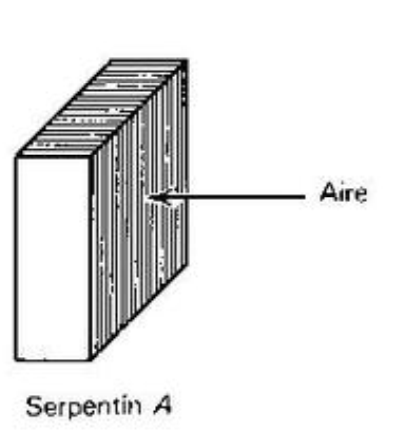
\includegraphics[width=\linewidth]{evaporadores/serpentin-a}
%					\end{subfigure}	
%					\begin{subfigure}{.3\linewidth}
%						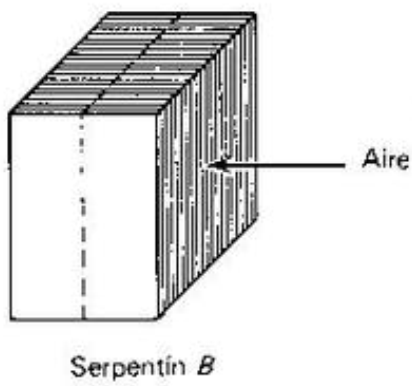
\includegraphics[width=\linewidth]{evaporadores/serpentin-b}
%					\end{subfigure}	
%					\begin{subfigure}{.3\linewidth}
%						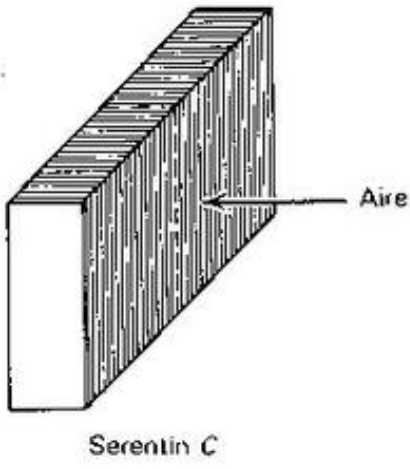
\includegraphics[width=\linewidth]{evaporadores/serpentin-c}
%					\end{subfigure}

					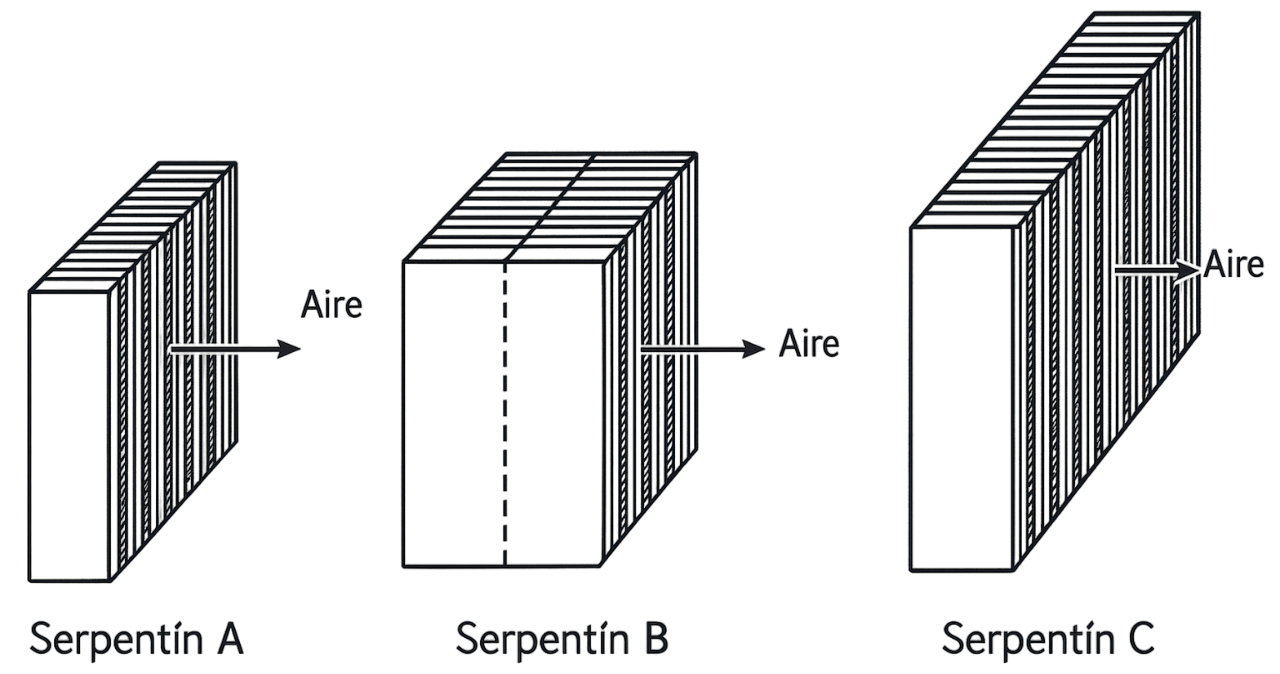
\includegraphics[width=.7\linewidth]{evaporadores/disposicion-serpentin}
					\caption{Los serpentines B y C tienen el doble de área superficial que el serpentín A. El serpentín C tiene doble área en el frente que el serpentín A o B.}
					\label{fig:disposicion-serpentines}
				\end{figure}
				
				En un serpentín de varias hileras, a medida que el aire pasa a través de estas, en cada hilera subsiguiente se tendrá una menor razón de transferencia de calor y funcionará con menos eficiencia que la hilera anterior. La METD es afectada cuando el área superficial del serpentín es aumentada al aumentar el número de hileras (profundidad). Suministrando aire a la misma velocidad, la METD a través de C será exactamente igual a la que se tiene a través de A, y por lo tanto la capacidad de C será el doble que la del serpentín A.
				
				\emph{Para la misma área superficial total, un serpentín largo, ancho y plano, será más eficiente que otro serpentín corto y angosto que tenga más profundidad}.
				
				Sin embargo, en muchas aplicaciones, el espacio físico es limitado, debiendo usarse arreglos con serpentines compactos. En algunas ocasiones, la pérdida de capacidad resultante por el incremento de la profundidad es compensada aumentando la velocidad del aire sobre el serpentín.
				
				Además, en algunas aplicaciones, es deseable tener serpentines profundos para propósitos de deshumidificación. Cuando el aire húmedo pasa por un serpentín cuya superficie tiene una temperatura por debajo del punto de rocío del aire, el vapor de agua condensa en forma de gotas. Al tener más hileras de tubos, el aire permanece más tiempo en contacto y su temperatura se aproximará más a la temperatura de la superficie del serpentín.
			
				
			\subsection{Circuitos en el evaporador}
			
			
			Los evaporadores de múltiples circuitos se utilizan cuando en el serpentín se produce una caída de presión demasiado grande para un solo circuito.
			
			Una caída de presión excesiva en el evaporador da como resultado una presión menor que la realmente necesaria en la succión de vapor a la entrada del compresor. Debido a esto, un buen diseño requiere de varios circuitos en el evaporador, de modo que la caída de presión sea la mínima necesaria para tener velocidades suficientes en el refrigerante, favoreciendo así una tasa alta de transferencia de calor al eliminar las burbujas de aire en la superficie del tubo y asegurando un buen retorno del aceite (aspectos tratados en la \autoref{sec:capacidad-evaporador}).
			
			En general, la caída de presión en el evaporador dependerá del tamaño del tubo, de la longitud y de la carga en el circuito. La carga\footnote{Por carga en el circuito se entiende la rapidez de flujo de calor a través de las paredes del tubo.} determina la cantidad de refrigerante que debe pasar a través del circuito. A mayor carga, mayor deberá ser la cantidad del refrigerante que fluya a través del circuito y mayor será la caída de presión.
			
			Se diseñan varias disposiciones de circuitos. En la bibliografía \cite[Sección 11.12]{dossat2004refrigeracion} se mencionan los siguientes circuitos:
			\begin{itemize}
				\item \textbf{Circuito serie simple.} El refrigerante sigue un solo camino a través de todo el evaporador. Los evaporadores con esta disposición, según la \autoref{fig:circuito-1}, trabajarán en forma satisfactoria dentro de ciertos límites de carga, ya que, cuando se exceda dicho límite la velocidad alcanzará valores no deseados provocando una gran caída de presión.
				\begin{figure}[h]
					\centering
%					\includegraphics[width=.5\linewidth]{circuito-1}
					\caption{Evaporador con un circuito refrigerante en serie.}
					\label{fig:circuito-1}
				\end{figure}
				
				\item \textbf{Circuito dividido.} A causa de la caída de presión al final de la disposición anterior se divide al circuito en dos trayectorias. Esto produce el efecto de reducir la velocidad del refrigerante a la mitad del valor y la caída de presión hasta la octava parte. Esto permitirá tener una mayor carga en el serpentín sin excederse de los límites. Como ejemplo, se muestra la \autoref{fig:circuito-2}.
				\begin{figure}[h]
					\centering
%					\includegraphics[width=.5\linewidth]{circuito-2}
					\caption{Evaporador con un circuito refrigerante dividido.}
					\label{fig:circuito-2}
				\end{figure}
				\item \textbf{Circuitos múltiples paralelos}. Se instalan cabezales en los extremos del evaporador para permitir que el refrigerante sea distribuido de manera simultánea a través de varios circuitos paralelos. Existen diferentes configuraciones posibles, dependiendo de la orientación de los circuitos y del sentido del flujo entre el aire exterior y el refrigerante. Es importante tener en cuenta la orientación, ya que influye directamente en la distribución de la carga, pudiendo provocar un reparto no uniforme del refrigerante entre los circuitos. Esto ocurre, por ejemplo, en la \autoref{fig:circuito-3}, donde la temperatura del aire que atraviesa el serpentín es mayor en los primeros circuitos y va disminuyendo a medida que se incrementa la profundidad, y en consecuencia, requieren de más refrigerante. En cambio, las \autoref{fig:circuito-4} y \autoref{fig:circuito-5} muestran una configuración donde solucionan este inconveniente.
				\begin{figure}[h]
					\centering
					\begin{subfigure}{.3\linewidth}
%						\includegraphics[width=.5\linewidth]{circuito-3}
						\caption{Evaporador de cuatro circuitos con cabezales de refrigerante. Con flujo cruzado de aire y refrigerante da como resultado una carga desigual.}
						\label{fig:circuito-3}
					\end{subfigure}
					\begin{subfigure}{.3\linewidth}
%						\includegraphics[width=.5\linewidth]{circuito-4}
						\caption{Evaporador con distribuidor de refrigerante y cabezal. Arreglo en contraflujo.}
						\label{fig:circuito-4}
					\end{subfigure}
					\begin{subfigure}{.3\linewidth}
%						\includegraphics[width=.5\linewidth]{circuito-5}
					\end{subfigure}
					\caption{Evaporador de cinco circuitos con cabezales de refrigerante. Arreglo en contraflujo y menor profundidad, permitiendo un diferencial de temperatura media mayor.}
					\label{fig:circuito-5}
				\end{figure}
			\end{itemize}
			
			% Acá se menciona al circuito simple, luego, una mejora de este es un circuito con refrigerante dividido (el circuito se divide en el punto que la velocidad alcanza la máxima permitida y luego se divide en dos trayectorias paralelas) Esto reduce la velocidad a la mitad y la caída de presión se reduce hasta la octava.
			% Evaporador de varios circuitos con cabezal a la entrada y salida. La desventaja es el desequilibrio de carga que hay en cada circuito, ya que la diferencia de temperatura es mayor en la primera hilera en contacto con la corriente de aire y se va reduciendo a mayor profundidad, y requiere mayor carga. Es imposible ajustar con una alimentacion simple de refrigerante para satisfacer a cada circuito sin subalimentar o sobrealimentar a los otros. Este tipo es más utilizado en sistemas inundados.
			% Mejora del anterior con sistema a contraflujo.
			% Evaporador con distribuidor a la entrada y salida (cabezales, supongo) pero el refrigerante circula en contraflujo con el aire. La transferencia de calor es mayor para este caso y la carga en los circuitos es regular. 
			
	
	\section{Sistemas de desescarche}
		
		La escarcha se forma en el evaporador debido al congelamiento de la humedad presente en el aire que lo atraviesa. Si bien el amplio espaciamiento entre las aletas permite inicialmente el paso del flujo de aire aun con algo de escarcha acumulada, con el tiempo esta se incrementa hasta bloquear el paso del aire. Además, la escarcha actúa como un aislante térmico, disminuyendo la eficiencia en la transferencia de calor. 
		
		Por esta razón, el serpentín requiere un proceso de descongelado, deshielo o desescarche periódico, que asegure un flujo de aire adecuado y una refrigeración eficiente.
		
		La acumulación de escarcha depende de las condiciones y la temperatura de evaporación del aire.
		
		Los métodos de descongelación pueden ser clasificados, según la fuente de calor utilizada, como
			\begin{itemize}
				\item \emph{desescarche natural},  utiliza el calor del aire que se tiene en el espacio refrigerado,
				\item \emph{desescarche con calor suplementario}, se obtiene con el calor suministrado de otras fuentes que no sean el calor del espacio refrigerado, como agua, salmuera, resistencias eléctricas y gas caliente.
			\end{itemize}
			
			Todos los métodos de desescarche natural requieren que el sistema (o el evaporador) esté detenido por un período de tiempo suficiente largo que le permita al evaporador elevar la temperatura hasta un nivel superior al punto de congelamiento.
			
			Independientemente del sistema que se utilice, excepto en el desescarche por aire, para realizar la descongelación hay que desconectar el ventilador del evaporador durante el proceso de descongelación, u ocurrirán dos cosas:
			\begin{itemize}
				\item El calor de la descongelación se transferirá directamente al espacio acondicionado.
				\item El aire acondicionado frío ralentizará el proceso de descongelación.
			\end{itemize}
			
			En general, las etapas para el proceso de deshielo son:
			\begin{itemize}
				\item Corte del suministro de refrigerante al evaporador. Se cierra la válvula que se tiene en la tubería del líquido.
			%	Orden de inicio de desescarche; puede ser manual o automática. Comienza cuando se detiene la inyección de refrigerante líquido en el interior del evaporador.
				\item Evaporación del refrigerante en el interior del evaporador. Este proceso se puede realizar continuando con la producción frigorífica si el compresor continúa funcionando debido a un retardo programado. Mientras que en otros sistemas se detienen el compresor y los ventiladores.
			%Evaporación del líquido del interior del evaporador; este proceso se puede realizar continuando con la producción frigorífica si programamos un retardo y mantenemos funcionando el compresor para mantener la presión baja en el evaporador y los ventiladores para favorecer el intercambio de calor. Sin embargo en otros sistemas, se detiene el compresor y los ventiladores con lo que se aumenta la duración del desescarche y la energía necesaria para este, pues habrá que suministrar energía no sólo para producir la fusión del hielo sino que también habrá que suministrar energía para producir la evaporación del refrigerante que queda en el interior del evaporador tras cesar la inyección.
			
			%Retardo 1; en algunos sistemas de desescarche, como los de gas caliente, será necesario efectuar un retardo para realizar ajustes en los sistemas que intervienen en el proceso (seguridad en la apertura y cierre de las válvulas).
				\item Este proceso puede realizarse con los ventiladores en funcionamiento, como en el caso del desescarche por aire, o, como es más habitual, deteniendo su funcionamiento para evitar la dispersión del calor.
			%Fusión del hielo; se trata de aportar energía para elevar la temperatura y lograr la fusión del hielo acumulado. Este proceso se puede realizar con los ventiladores funcionando, como en los desescarches por aire, o como es habitual, parando los ventiladores; esto dependerá de las características de la cámara o mueble frigorífico. En los sistemas modernos en los que el tiempo se define por la sonda final de desescarche, se suele programar una duración máxima de desescarche y si no se alcanzara la temperatura deseada en el tiempo fijado, se lanzará una alarma al sistema. Esto puede producirse por una avería en el sistema de desescarche (resistencias) o por no haber detenido la inyección de líquido. También se puede producir esta anomalía por haber mantenido la puerta de la cámara abierta durante largos periodos de tiempo o por alguna rotura en los cerramientos que provoque infiltraciones de aire exterior.
			
			%Retardo 2; en este punto, algunos sistemas necesitan efectuar un retardo para realizar ajustes en los sistemas que intervienen en el desescarche (islas de congelados).
				\item Drenaje del evaporador. Es necesario establecer un tiempo adicional para facilitar la evacuación de los condensados generados tras la fusión del hielo.
			%Tiempo de goteo o drenaje del evaporador; es necesario dar un tiempo para facilitar la evacuación de los condensados producidos tras la fusión del hielo debido a la apertura de las válvulas de aspiración en desescarche por gas caliente.
				\item Inyección de refrigerante. En esta etapa se reintroduce el refrigerante en el evaporador. Si queda agua remanente tras el desescarche, esta puede volver a congelarse al restablecerse las condiciones de funcionamiento.
			%Inyección de refrigerante; se vuelve a introducir refrigerante en el evaporador, y comienza a congelarse el agua que pueda quedar mojando las aletas y los tubos.
				\item Retardo en el funcionamiento de los ventiladores. Es importante llevar a cabo este paso una vez iniciada la inyección de líquido, para evitar que el agua presente sobre las aletas sea arrastrada y proyectada hacia el espacio refrigerado.
			%Retardo de conexión de los ventiladores; es importante retardar la conexión de los ventiladores tras comenzar la inyección de líquido para evitar que el agua que pueda estar mojando las aletas sea proyectada hacia la cámara. Este retraso permite que esta agua se congele. La conexión de los ventiladores se producirá al sobrepasar el tiempo indicado en el temporizador o bien cuando se detecte una temperatura por debajo del punto de congelación en la sonda final de desescarche. El retraso de conexión de los ventiladores también puede ser consecuencia de que en grandes evaporadores de cámaras de temperaturas muy bajas, se produce la conexión de los ventiladores estando el evaporador muy caliente, se puede predecir una onda expansiva por choque térmico al ponerse en contacto aire frio de la cámara y aire caliente del evaporador.
			\end{itemize}
			
		\subsection{Descongelamiento por aire}
		
		El método utiliza el calor del aire que se tiene en el espacio refrigerado para fundir el hielo del evaporador. Consiste en apagar el sistema de refrigeración y permitir que el aire no refrigerado circule sobre el serpentín. Dado que el aire se encuentra a una temperatura superior a la de la escarcha, facilita su derretimiento. Este tipo de descongelamiento por aire puede ser más lento que otros métodos y su eficacia dependerá tanto de la temperatura del aire como de la cantidad de escarcha acumulada.
		
		Este método resulta útil y es utilizado para temperaturas del evaporador superiores a 1°C.
		
		\subsection{Descongelamiento por agua}
		
		En el método de desescarche por agua se rocía agua sobre el serpentín del evaporador para derretir la escarcha. Generalmente, se sigue el siguiente procedimiento:
		\begin{enumerate}
			\item Se cierra la válvula del suministro de refrigerante y es evacuado del evaporador.
			\item Se detiene el compresor y los ventiladores para que el agua atomizada no ingrese al espacio refrigerado.
			\item Inicia el funcionamiento de los atomizadores de agua hasta que el evaporador sea deshielado, lo cual, según \cite{dossat2004refrigeracion}, requiere aproximadamente 4 a 5 minutos.
		\end{enumerate}
		
		Cuando se utiliza salmuera o una solución anticongelante, la solución no se desperdicia sino que regresa a un depósito para después hacerla circular.	
		
		Para evaporadores cuya temperatura baja hasta aproximadamente $-40$ °C, el deshielo se efectúa rociando agua sobre la superficie de los serpentines del evaporador. Para evaporadores cuya temperatura sea inferior a $-40$ °C, podrá sustituirse el agua por salmuera o alguna solución anticongelante.
		
		\subsection{Descongelamiento eléctrico}
		
		La descongelación eléctrica se realiza utilizando calentadores eléctricos situados en el evaporador. El compresor se detiene y estos calentadores se activan para realizar la descongelación, permitiéndoseles trabajar hasta que haya derretido todo el hielo del serpentín.
		
		\begin{figure}[h]
			\centering
%			\includegraphics[width=.5\linewidth]{descarche-electrico}
		\end{figure}
		
		\subsection{Descongelamiento por gas caliente}
		
		El descongelamiento por gas caliente tiene muchas variaciones, pero esencialmente, en este método se utiliza como fuente el calor interno del sistema proveniente del gas descargado por el compresor. 
		
		
		Se instala una válvula solenoide en un tubo de desviación instalado entre la descarga del compresor y la entrada del evaporador. Cuando la válvula está abierta, el gas expandido circula desde el compresor hacia el evaporador cediendo su calor al evaporador frío y se condensada. Parte del refrigerante condensado permanece en el evaporador, mientras que el resto regresa al compresor donde es evaporado por el calor de la compresión y recirculado al evaporador. 
		
		
		Una limitante de este método es que a medida que se da el descongelamiento, más líquido permanece en el evaporador y menos retorna al compresor, con el resultado de que el sistema agote su calor antes que el evaporador esté completamente deshielado. Otra desventaja es la posibilidad de que una capa pesada de refrigerante líquido regrese al compresor y cause daño en este.
		
		Estos inconvenientes se puede resolver proporcionando algunos medios para evaporar el refrigerante que condensa en el evaporador y los medios empleados distinguen a un método de otro.
		
		\subsection{Descongelamiento por inversión de ciclo}
		
		Se basa en el principio del ciclo invertido (bomba de calor), en donde el condensador puede utilizarse como serpentín para evaporar al refrigerante que se condensada en el evaporador durante el ciclo de desescarche. Para este tipo de operación se utilizan válvulas de 4 vías (\autoref{fig:valvula-4-vias}).
		
		La \autoref{fig:deshielo-bomba-calor} se muestra un esquema de flujo para las operaciones normal y de descongelamiento, respectivamente.
%		
%		\begin{figure}[h]
%			\begin{subfigure}{.4\linewidth}
%				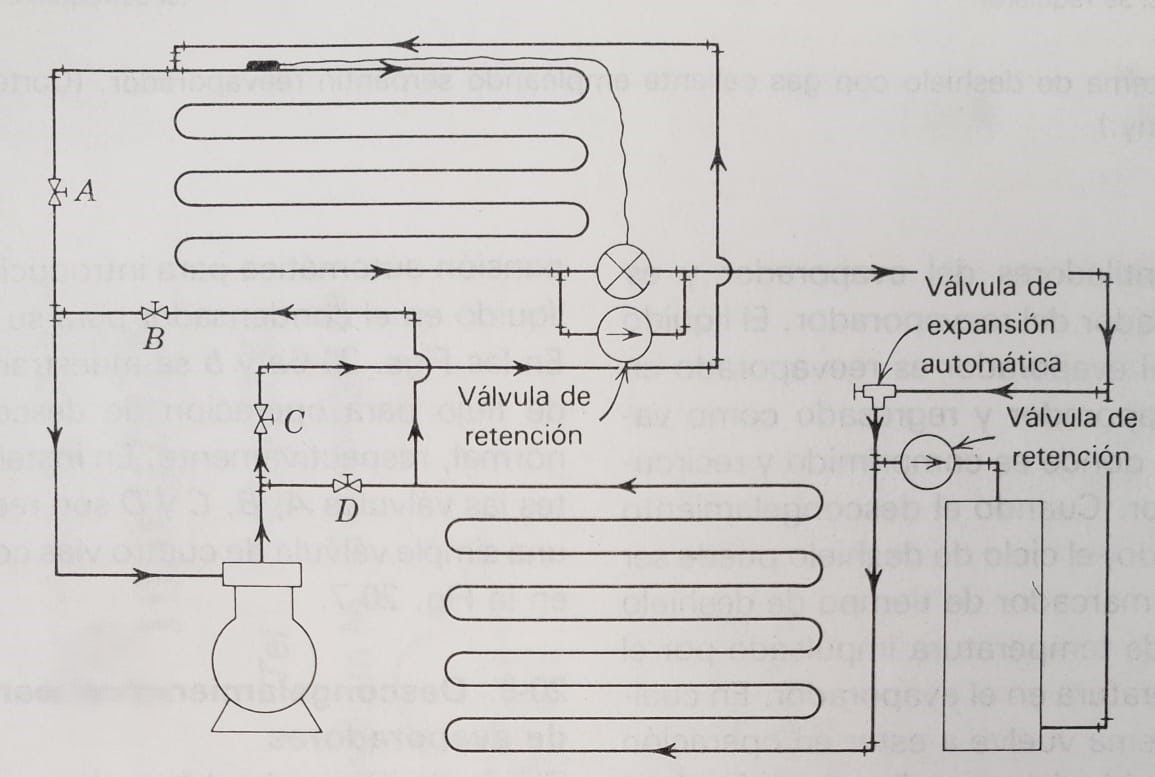
\includegraphics[width=\linewidth]{inversion-1}
%				\caption{Operación normal}
%				\label{fig:inversion-1}
%			\end{subfigure}
%			
%			\begin{subfigure}{.4\linewidth}
%				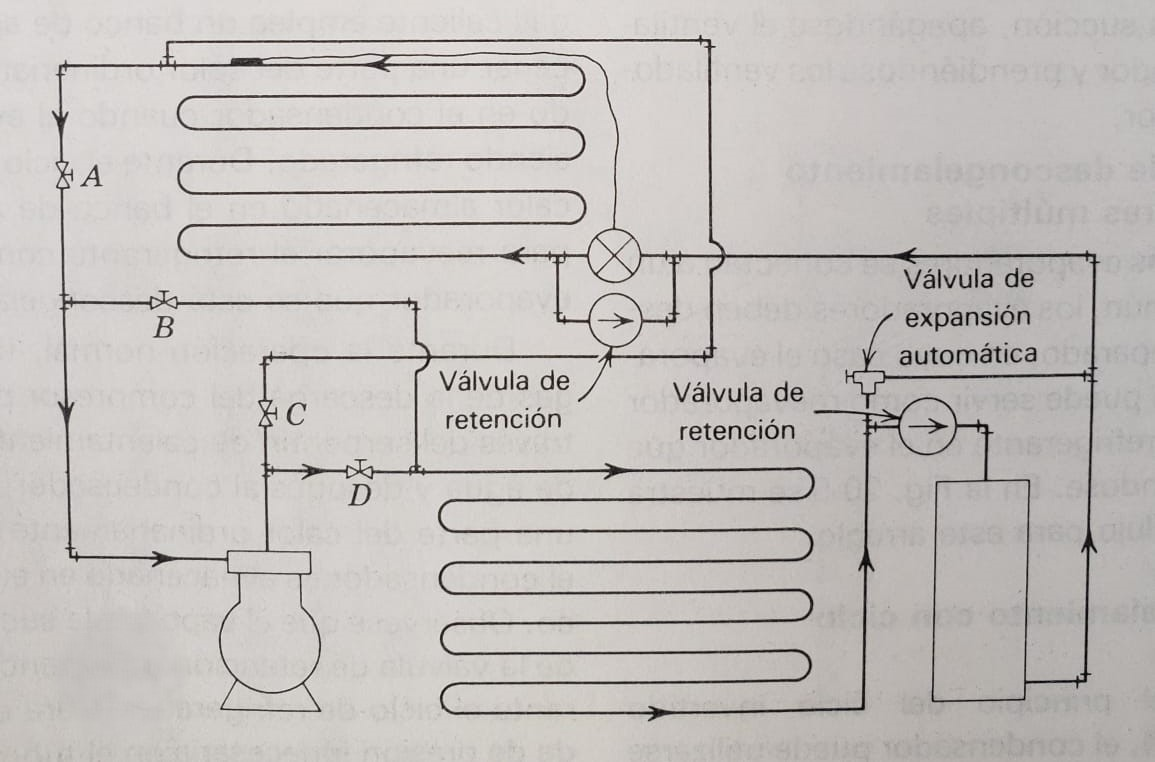
\includegraphics[width=\linewidth]{inversion-2}
%				\caption{Operación de descongelamiento}
%				\label{fig:inversion-2}
%			\end{subfigure}
%			\caption{Esquema de flujo para un sistema de descongelamiento por ciclo invertido.}
%			\label{fig:deshielo-bomba-calor}
%		\end{figure} 
		
		
		\begin{figure}[h]
			\begin{subfigure}{.35\linewidth}
				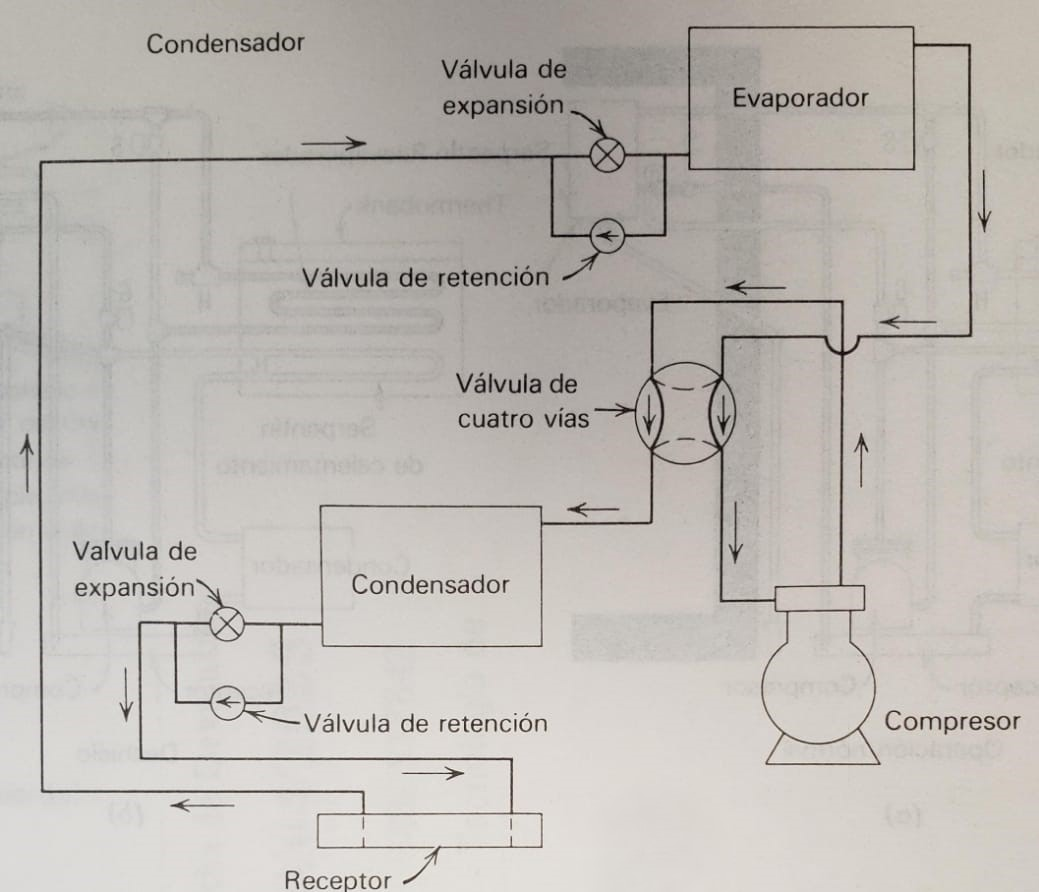
\includegraphics[width=\linewidth]{evaporadores/inversion-3}
				\caption{Operación normal}
				\label{fig:inversion-3}
			\end{subfigure}
			
			\begin{subfigure}{.35\linewidth}
				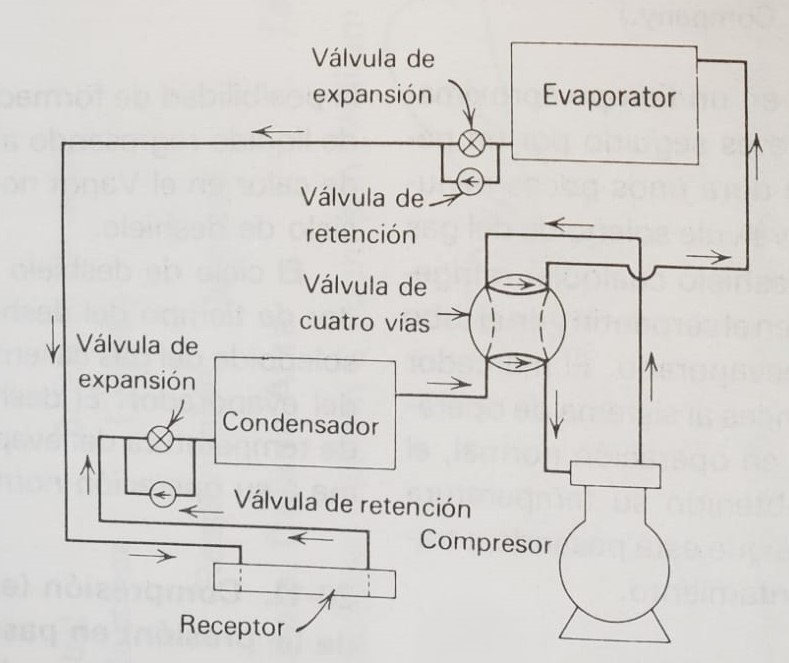
\includegraphics[width=\linewidth]{evaporadores/inversion-4}
				\caption{Operación de descongelamiento}
				\label{fig:inversion-4}
			\end{subfigure}
			\caption{Esquema de flujo para un sistema de descongelamiento por ciclo invertido empleando una válvula de cuatro vías.}
			\label{fig:deshielo-bomba-calor}
		\end{figure} 
		\begin{figure}[h]
			\centering\caption{Válvula de cuatro vías.}
			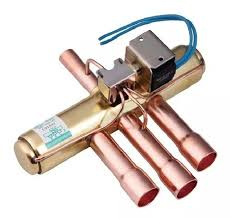
\includegraphics[width=.5\linewidth]{evaporadores/images}
			\label{fig:valvula-4-vias}
		\end{figure}
		
	\section{Diseño y selección de evaporadores}
		
		Uno de los principales parámetros para el diseño de un evaporador es su capacidad de enfriamiento, vista en la \autoref{sec:capacidad-evaporador}. Otro de los factores más importantes a considerar en cualquier aplicación para la selección del evaporador adecuado es la \acrlong{dt}, ya que depende del tipo de aplicación y se determina en función de las condiciones de temperatura y humedad requeridas en el espacio.
		
		
		La selección del evaporador se realiza consultando los catálogos de los fabricantes. Debido a que calcular todas las variables que afectan su rendimiento no resulta práctico, generalmente, se determina a partir de ensayos reales. Aunque el método puede variar según el tipo de evaporador y el fabricante, las diferencias no suelen ser significativas y cada catálogo incluye instrucciones para interpretar correctamente los datos.
		
		\subsection{Dt del evaporador}
		
		El salto térmico del evaporador ($Dt$) es la diferencia de temperaturas entre la del fluido refrigerante, evaporándose en el interior del evaporador, y la del fluido a enfriar. 
		\begin{equation}
			Dt = t_c - t_e
		\end{equation}
		Donde 
		\begin{itemize}
			\item $t_e$ corresponde a la temperatura en el evaporador, o temperatura de evaporación,
			\item $t_c$ es la temperatura de la cámara o de diseño.
		\end{itemize}
		
		La Dt está condicionada por el tipo de aplicación debido a que tiene una gran influencia sobre la humedad relativa de la cámara, que a su vez está determinada por el tipo de producto\footnote{Cada producto tiene su propia temperatura y humedad relativa para poder ser mantenidos en óptimas condiciones de conservación o congelación.} en su interior. A partir del tipo de aplicación, se define la Dt del evaporador, lo cual permite establecer la temperatura de funcionamiento del mismo.
		
		El modelo de evaporador se debe elegir a partir de las tablas que figuran en los catálogos de los fabricantes, ya que es aquí donde aparecen todos los parámetros y factores de corrección que permiten indicar cuál es el más adecuado. Cada fabricante cuenta con sus propias tablas de selección y suelen ser diferentes entre un fabricante y otro.
		
		\subsection{Relación entre la Dt y la humedad relativa}
		
		La conservación de alimento y otros productos en condiciones óptimas de refrigeración, depende no únicamente de la temperatura del espacio refrigerado sino también de la humedad relativa en dicho espacio. Cuando es muy baja la humedad, se tiene una deshidratación excesiva. En caso contrario, cuando la humedad relativa es muy elevada, favorece el crecimiento de bacterias, hongos y se propicia una formación de una delgada capa de lama sobre el producto, y este último se da sobre todo en carnes.
		
		El factor más importante que regula la humedad es la $Dt$ del evaporador. Mientras menor sea esta diferencia de termperatura, mayor será la humedad relativa en el espacio refrigerado. Así mismo, a mayor Dt del evaporador, menor será la humedad relativa. La \autoref{fig:curva-hr-dt} muestra la relación entre la humedad relativa presente en la cámara y el salto térmico del evaporador.
		
		\begin{figure}[h]
			\centering
			%			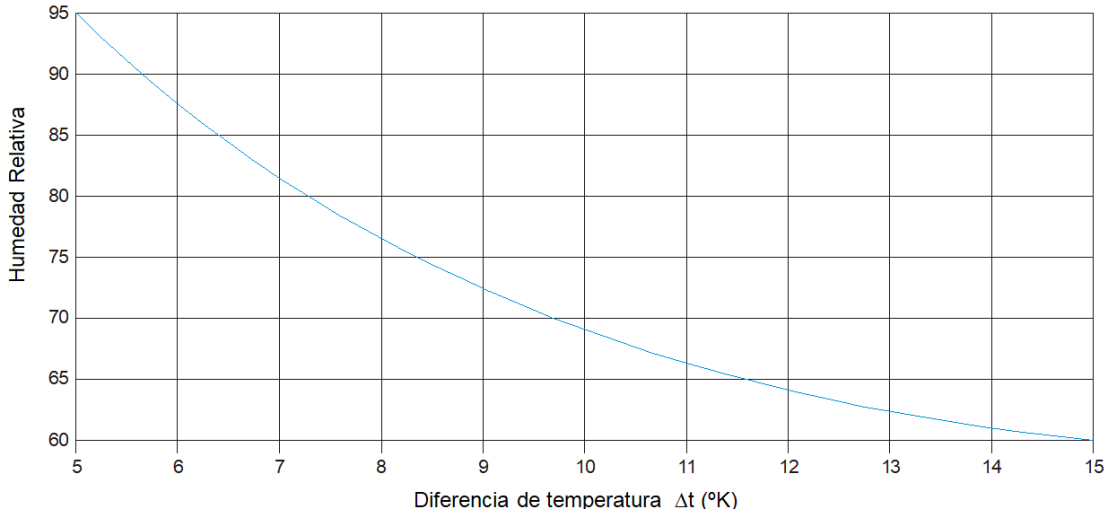
\includegraphics[width=.5\linewidth]{curva-hr-dt}
			\caption{Relación entre el salto térmico y la humedad relativa en la cámara.}
			\label{fig:curva-hr-dt}
		\end{figure}
	\section{Factor de By-pass}
	\section{Control de temperatura y humedad relativa}
%	Unidad 4 - aire humedo y psicro 2022 pdf
		\subsection{Control en verano}
		\subsection{Control en invierno}
%	\section{Variaciones en la carga}
